% LAB 2:
% State space modeling

\Opensolutionfile{StaVarSolutions}
% \begin{solstavar}
% \end{solstavar}

\chapter{State Variable Modeling} \label{ch.StaVar}

The purpose of this session is to introduce the basics of state variable modeling known as ``state space'' techniques.  The state space technique is a unified time-domain formulation that can be utilized for the analysis and design of many types of systems.  It can be applied to linear and nonlinear continuous-time and discrete-time multivariable systems.

\section{Pre-Lab Assignment}
An introduction to the basics of state variable modeling can be found in Appendix~\ref{app.statespace}.  Read the Appendix and familiarize yourself with state variable creation as well as the analytical and numerical methods of solution.

\section{Laboratory Procedure}
Complete the following case study after reading Appendix~\ref{app.statespace}.

\begin{figure}[hbt]
\centering
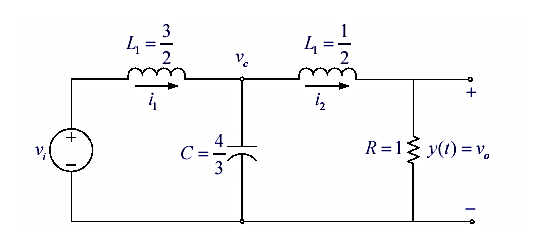
\includegraphics[width=3.4in]{thirdorderLPfilter}
\caption{\footnotesize
        Third-order low-pass filter
        \label{fig.statespacelab.thirdorderLPfilter}
        }
\end{figure}

\begin{enumerate}
\item The circuit shown in Figure~\ref{fig.statespacelab.thirdorderLPfilter}
    is a third-order Butterworth filter.  Select appropriate state variables and obtain the state and output equations.  Treat the output, $y(t)$, as the voltage across the resistor.\\
    The general idea is to express the differential equations that describe the circuit as a system in matrix form.  With this in mind, the following notes may be helpful:
        \begin{itemize}
        \item In the absence of all capacitor and voltage source loops and all
            inductor and current source cut-sets, the number of state variables is equal to the number of energy storage elements.
        \item Appropriate state variables may be the voltage across the
            capacitor and the current in the inductors.
        \item Write a node voltage equation for every node touching a
            capacitor.  Also, consider writing loop equations in terms of the inductor currents for loops containing inductors.
        \end{itemize}
\item Write a script m-file and use the Control System Toolbox functions
    \verb=ss= and \verb=ltiview= to form the state model and its step response.  Also, use \verb=ss2tf= to obtain the filter's transfer function.\\
    Run the m-file.  Right-click on the LTI Viewer and use Characteristics to display all of the time-domain specifications.  Be sure to look at both the step- and impulse-response plots.  \\
    Right-click on the LTI Viewer again and from the Plot Type list, select ``Bode.''  From the File menu, select ``Print to Figure'' to obtain a figure plot capable of being edited.  Click on the magnitude response and hold and drag to display the corner frequency at -3~dB.  Now drag to display the attenuation at 10~rad/sec.\\
    Summarize the step response characteristics and the filter transfer function.  Comment on the filter frequency response characteristics.
\end{enumerate}

\Closesolutionfile{StaVarSolutions}